\chapter{Background}
\label{c:background}
Our traffic light detection system uses sensor fusion to estimate the motion and orientation of a smartphone and image processing in an estimated subpart of a video frame to detect the traffic lights. 
We use some existing techniques for these stages. 
In this section, we provide an overview of these techniques. 

%% In this chapter, we discuss the background of our system.
%% The main approach of our system is to improve the traffic light detection using smartphone sensor.
%% In the first part of this chapter, we discuss the inertial sensor of Android and sensor fusion.
%% Later we discuss the traffic bulb detection process.

\section{Inertial sensor of smartphone}
Virtually all smartphones come with a set of inertial sensors. These include an accelerometer, a gyroscope, and a geomagnetic field sensor. 
Below, we provide a brief overview of these sensors. 


\subsection{Accelerometer}
The accelerometer is one of the motion sensors in a smartphone.
Smartphones nowadays have three axis accelerometer, which can measure acceleration along the three axes of a smartphone's reference frame.
The accelerometer does not measure free fall acceleration.
Instead, it measures the forces that are applied to the accelerometer itself.
For example, when the phone is on the table, it measures the gravitational acceleration $g$ because this is proportional the accelerometer's weight.
\todo{this is not clear}.

Figure \ref{f:acc} shows the reference coordination frame of an accelerometer in an Android smartphone.
The accelerometer measures the acceleration with respect to the reference frame and returns a vector $[a_x, a_y, a_z]$.
Here, $a_z$ points perpendicular with respect to the smartphone's screen and $a_x$ and $a_y$ point right and up in the phone's planes respectively as shown in Figure \ref{f:acc}.

\begin{figure*}[!ht]
\centering
\subfloat[Accelerator coordination] {\label{f:acc}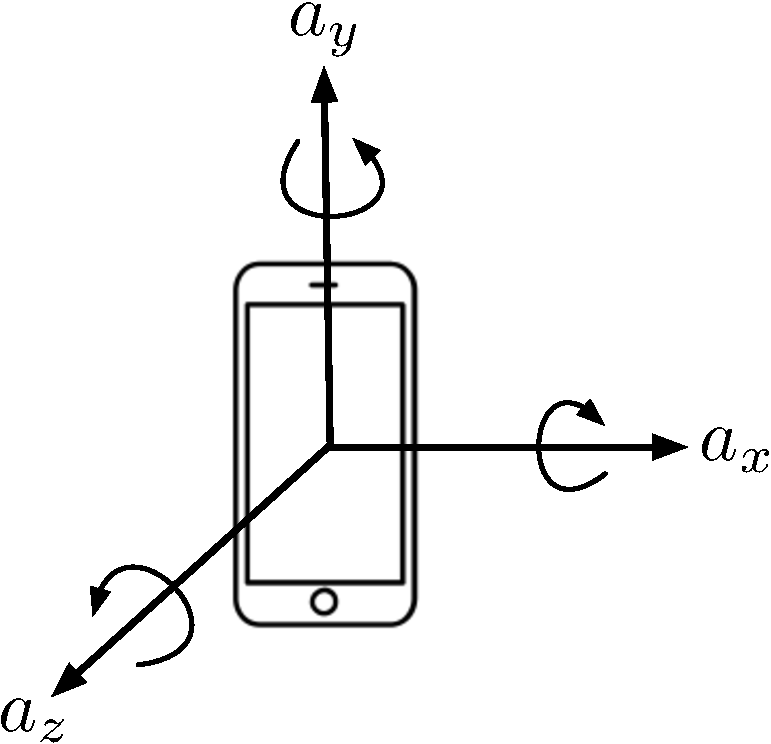
\includegraphics[width=2.5in]{figures/coord_acceleration.pdf}}
\hfill
\subfloat[Gyroscope coordination] {\label{f:gyro}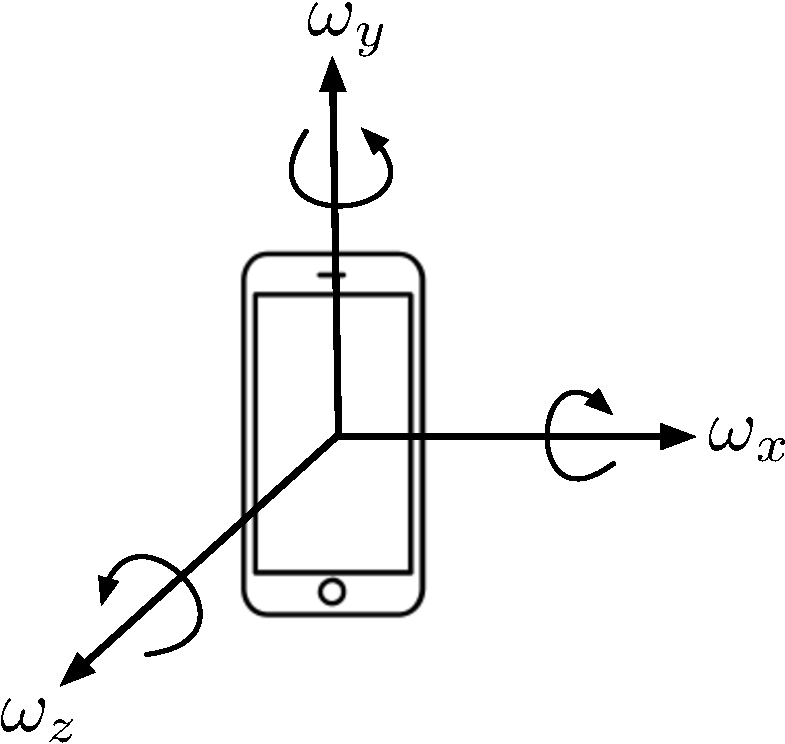
\includegraphics[width=2.5in]{figures/coord_omega.pdf}}

\caption{Smartphone reference coordination system.}
\label{f:coord_dia}
\end{figure*}

\subsection{Gyroscope}
The accelerometer is another motion sensor in a smartphone.
The gyroscope measures the rate of rotation or the angular velocity of rotation along the three axes of a smartphone's reference frame.
%This is also a motion sensor of smartphone like an accelerometer.
The gyroscope is a MEMS (Micro-Electro-Mechanical Sensing) sensor that uses vibrating elements to measure Coriolis effect \todo{cite}.
When a smartphone rotates, there is a change of direction in the vibrating elements because of the Coriolis force.
A MEMS gyroscope measures these variations along the three axes to estimate the rate of rotation.
Gyroscopes are very responsive to small rotations and can measure the variation in the rate of rotation smoothly.

Figure \ref{f:gyro} shows the reference coordination frame of a gyroscope on an Android phone.
The coordination frame for the gyroscope is same as the coordination frame of accelerometer described above.
The gyroscope measures the angular velocity with respect to the reference frame and returns a vector $[\omega_x, \omega_y, \omega_z]$.

%% The angular velocity of rotation $\omega_z$ points towards the outside of screen face, that is perpendicular to the phone plane, which is the angular velocity of phone's rotation in the X-Y plane.
%% The rate of rotation $\omega_x$ and $\omega_y$ is along with the phone plane, which is the angular velocity of phone's rotation in the Y-Z plane and the Z-X plane respectively.

\subsection{Geomagnetic field sensor}
Geomagnetic field sensor is a position sensor of the smartphone.
It helps to determine the smartphone's physical position in the Earth's reference frame.
%Geomagnetic field sensor measures the change of the magnetic field and estimates the magnetic field at earth's point to find the declination from the true North.
Geomagnetic field sensor measures the change of the magnetic field and estimates the declination of a smartphone with respect to the true North. \todo {what is declination. Also, is there any difference between true north and magnetic north?}
It provides the geomagnetic field strength along the three coordination axes of the reference frame.
\todo {how three axis is relevant? Isn't it a single number describing rotation compared to the north}

\subsection{Orientation}
Each sensor described in the previous section has its own strength and weakness.
The gyroscope is fast, accurate and reliable.
It is also very responsive to a small rotation.
As a result, it can track the change of rotation rapidly.
However, the gyroscope can not measure gravity. \todo{should go after accelerometer?}
So with the accelerometer, it can provide a better rotation or motion of the sensor in application's frame reference. \todo{how accelerometer helps here?}
Additionally, to obtain the position of a smartphone in the Earth's reference frame, we need to combine the gyroscope and accelerometer data with geomagnetic field sensor.

Android Sensor API \todo {cite} provides the orientation of the phone with respect the reference frame described before by fusing the data from the accelerometer, gyroscope, and magnetic sensor. 
This orientation contains the pitch, roll, and azimuth of the smartphone. 
%Another motion sensor in android, rotation vector, use this three sensor data to report the orientation of the device in vector form along the axis of the reference frame.

%This rotation vector provides the axis of the system and the angle of rotation from these axes.
%

\begin{figure}
\centering
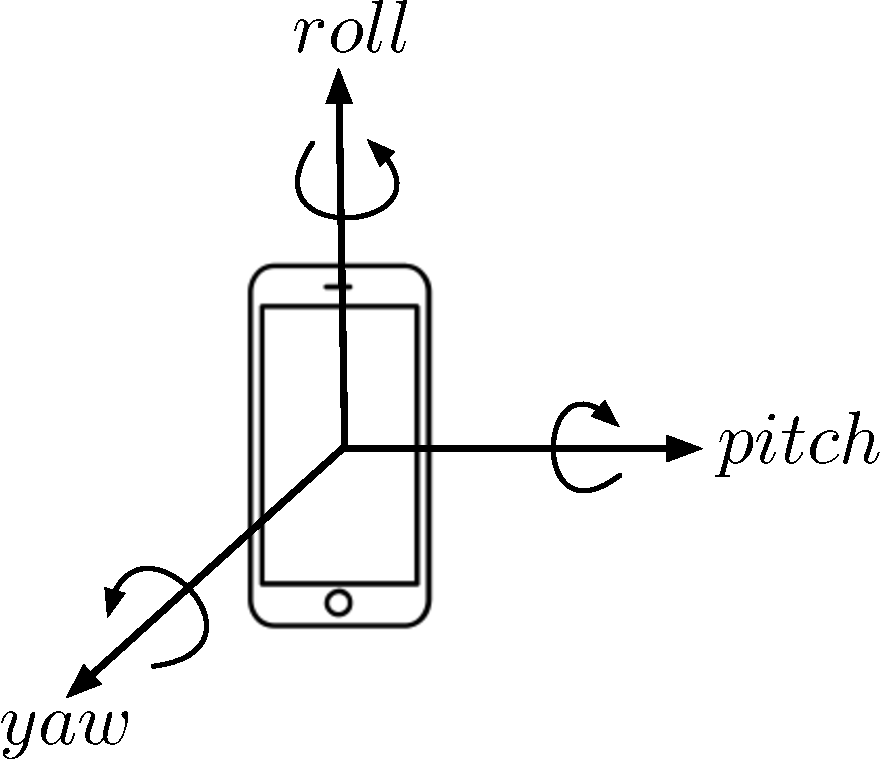
\includegraphics[width=3.8in]{figures/roll_pitch_yaw.pdf}
\caption{Orientation of the smartphone}
\label{f:rpy_dia}
\end{figure}

\ref{f:rpy_dia} shows the orientation of a smartphone with respect to the smartphone's coordination frame.
Here, the pitch is the degree of rotation about the X axis.
Pitch is the angle between the plane parallel to the smartphone and parallel to the ground. \todo{clarify, parallel twice is ambiguous.}
If the smartphone's top edge inclines to the ground the pitch will be positive and vice versa.
\todo{overall below is confusing to read. May be table is better}
The range of pitch value is -180 degrees to 180 degrees.
Roll is the rotation angle with respect to the Y axis.
This is the angle between the plane perpendicular to device and perpendicular to the ground.
If device's left edge inclines to the ground roll value is positive.
The range of roll is from -90 degrees to 90 degrees.
Azimuth is the rotation angle with respect to the Z axis.
If the device is faced to the Earth's North then the azimuth is 0 degree.
Azimuth is 90 degree at the Earth's east, 180 degrees at the Earth's south, and 270 degrees at the Earth's west.


\section {Image Processing}
We process each video frame using computer vision techniques to detect traffic lights. 
Below, we provide a brief overview of these techniques. 

\subsection{Color Space}
RGB \todo{cite} and HSV \todo{cite} are two primary color spaces that are used in image processing and computer vision.
RGB defines a color as a combination of the three primary colors red (R), green (G), and Blue (B).
Hence, RGB is an additive color space.
%RGB color space describes colors with the amount of red, green and blue color presents on that frame.
\ref{f:rgb} shows the model of RGB space.
It shows that any color of this cube is a combination of red, blue, and green.

HSV color space describes color in terms of Hue, Saturation, and Value.
HSV color space is similar to the way human perceive a color.
It separates the color information from the intensity/brightness.
The hue is the continuous representation of the color type. \todo{confusing}
In HSV, hue is an angle from 0 to 360 degree. 
\todo{make a table?}
However, the OpenCV \todo{cite} represents color values using the range from 0 to 255. 
Hence, the OpenCV converts the original range to 0-180.
Every color can be represented by a different value of Hue.
Saturation represents the vibrancy of the color.
The ranges for saturation is from 0 to 255.
The lower value of saturation represents gray tone in a color and higher value of a saturation represents a primary color.
The Value represents the brightness of a color.
The range of the Value is from 0 to 255.
A lower Value means less bright color and vice-versa.
A Value of 0 represents the black color.

\begin{figure}[htbp]
\begin{minipage}[t]{0.45\linewidth}
    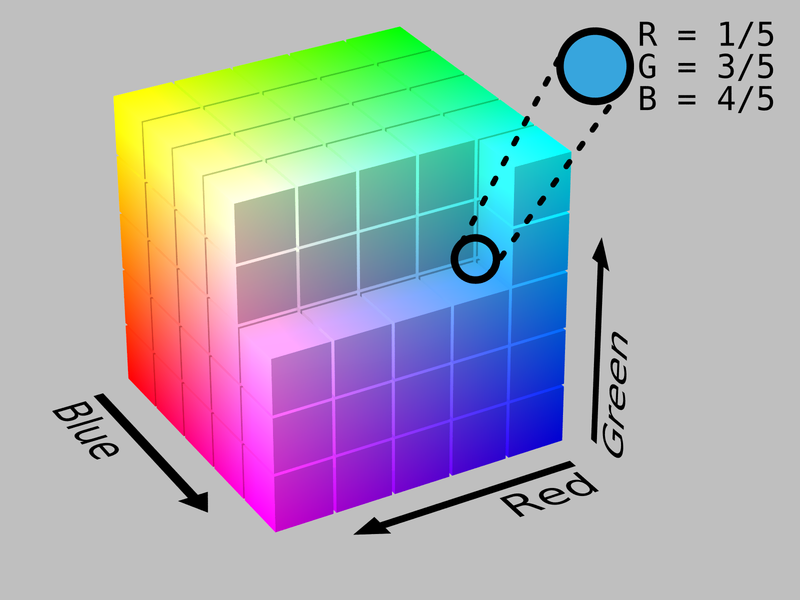
\includegraphics[width=\linewidth]{images/RGB.png}
    \caption{RGB color space}
    \label{f:rgb}
\end{minipage}
    \hfill
\begin{minipage}[t]{0.45\linewidth}
    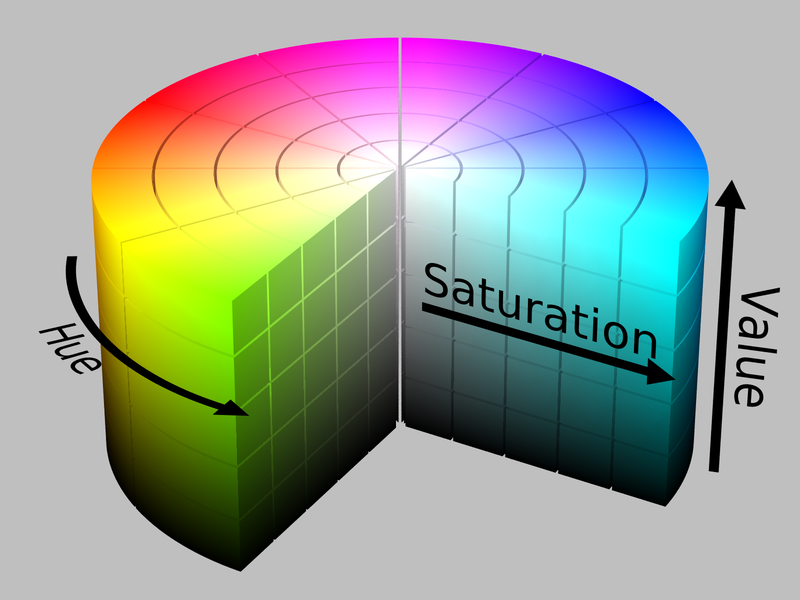
\includegraphics[width=\linewidth]{images/HSV.png}
    \caption{HSV color space}
    \label{f:hsv}
\end{minipage} 
\end{figure}

\ref{f:hsv} shows the cylindrical model of HSV color space.
Here, the Hue is the central part.
The radius of this cylinder represents Saturation and the height of the cylinder represents the Value.

\subsection{Hough Circle Transform}
Our system detects the circular bulb in a traffic light using the Hough circle algorithm \cite{houghcir_alg}.
The Hough circle algorithm first detect the edges in a video frame.
It uses Canny method \todo {cite} for edge detection.
\todo{can you make it more clear?}
Then, at every edge pixel, it generates a circle.
To find the intersection of these circles, Hough method uses an accumulator matrix.
If a circle passes through the grid of the accumulator matrix, it increases the voting number of the grid.
The position of the local maxima of this accumulator matrix provides the corresponding circle's centers.







